\documentclass[twocolumn]{article}

% packages
\usepackage{amssymb} 
\usepackage{amsmath}
\usepackage{algorithm}
\usepackage{algpseudocode}
\usepackage{graphicx}

% commands
\newcommand{\set}[1]{\left\{#1\right\}}
\newcommand{\seq}[1]{\langle #1 \rangle}
\newcommand{\type}[1]{\mathrm{#1}}
\newcommand{\mat}[1]{\mathbf{#1}}
\newcommand{\hamming}[2]{\textsc{Hamming}(#1, #2)}

\newcommand{\fig}[1]{Fig.~#1}
\newcommand{\subfigure}[1]{\textbf{(#1)}}
\newcommand{\sect}[1]{Sec.~#1}
\newcommand{\tab}[1]{Table~#1}
\newcommand{\alg}[1]{Alg.~#1}
\newcommand{\lst}[1]{List.~#1}
\newcommand{\eqn}[1]{Eq.~#1}
\newcommand{\thm}[1]{Thm.~#1}
\newcommand{\lem}[1]{Lemma~#1}
\newcommand{\corr}[2]{\text{Corr}\left[#1, #2\right]}

% bibiliographic info
\title{Pattern formation by evolution of cellular automata}
\author{Alex Garruss \and Casey Grun}
\date{\today}

\begin{document}
\maketitle

% =============================================================================
\section{Abstract}

Biological systems are able to develop exquisitely complex patterns; the existance of very simple computer programs that can produce highly complex behavior suggest that the rules underlying these natural pattern formation processes may be very simple. In this work, we attempt to use an evolutionary algorithm to explore the space of initial conditions for an elementary cellular automaton (Rule 110), known to be Turing complete. We show that, despite the fact that the mapping between ``genotypes'' (initial conditions of a cellular automaton) and ``phenotypes'' (final states of the automaton) is complex, regions of local smoothness exist, and very simple patterns can be evolved by selection pressure. These results suggest that certain problems, despite having complicated genotype-to-phenotype mappings, may still be amenable to solutions by genetic algorithms if a fitness landscape can be formulated that is locally smooth. Finally, we discuss the applicability of these results to biological pattern-formation and general evolutionary processes.

% =============================================================================
\section{Introduction}

Elementary two-dimensional cellular automata are simple computational programs defined by a rule set and seeded with an initial condition state.  The rule set determines the current value of a cell given a local neighborhood of previously computed cell states.  The initial condition space can significantly impact the immediate computational context, drastically affect the overall state of the automata during computation, and ultimately determine the diversity of output states for a given fixed rule set and output definition.
A traditional computer programming paradigm is frequently ``top-down'' in the sense rational paradigms and requirements of exactness for results (top-level outcomes) are directly achieved by design of lower-level procedures.  In contrast, genetic programs as they exist through evolution tend to arise from the natural ``bottom-up'' paradigm, beginning with simple cellular interactions that form higher-order structures and patterns.
Cellular automata provide a computational paradigm to explore simple rules and resulting complexity.  Cellular automata states are abstract and allow granularity corresponding to any part of an object or process.  Rule 110 was shown \cite{Cook:2004tt} to be Turing complete by showing equivalence of the automata to cyclic tags, previously proven to be complete.  This feature of the rule set implies a capability to harbor a vast diversity of output configurations, and potentially capable of harboring structures or patterns within the computed landscape of the running automata.

Emerging studies over the past several decades have looked to various cellular automata to describe patterns in biology.  In 1999 the theoretical biologist Andreas Deutsch proposed a migration automata to model cellular movement and morphogenetic pattern formation. \cite{Deutsch:1999wh} After building and refining a model (although not an elementary CA as proposed in the project), he describes the process of inferring simulated outcomes from observing rule definitions themselves.  For our proposed work, we expect to learn information about selected automata rule sets or initial conditions after computational evolution.  Deutsch proposes further morphogenetic description possibilities via simple automata to investigate other areas of pattern formation such as body formation.  We agree with his proposition, noting the sequential, hierarchical, and spatially-local pattern formation of the fly embryo. \cite{Clyde:2003fy}  Furthermore, Deutsch suggests extending the model to link proper pattern formation to subsequent cell decisions, such as differentiation.  This suggestion could be interpreted in our proposed framework to shift rule sets upon a resulting pattern of interest during computation.

Other groups (reviewed by Ermentrout et al. \cite{Ermentrout:1993ky}) have also approached pattern formation, along with areas in neurobiology and population dynamics.  Our approach differs dramatically in most cases since most of the previous groups rationally target mathematical models for a task at hand, whereas we propose to evolve input conditions to an elementary cellular automaton in an non-rational, unsupervised way. 

Our project is to use an evolutionary algorithm to explore the process of computational pattern formation using cellular automata. We take inspiration from Stephen Wolfram’s program to exhaustively explore the behavior of each possible rule set for an elementary cellular automaton, \cite{Wolfram:2002wq} and would like to perform a similar such exploration of the space of initial conditions for such an automaton. Rather than exhaustively enumerate and then examine all possible initial conditions, we will take a restricted, evolutionary approach. Specifically, we will attempt to answer the question: can we use evolutionary algorithms to generate initial conditions (``genotypes'') for a cellular automaton that can produce arbitrary output patterns (``phenotypes'')? Our starting point is Rule 110. 

There are several important challenges in addressing this question:
\begin{description}
\item[Formulation of the evolutionary process] --- It is not immediately obvious how to map cellular automata on to a genotype space which can be evolved; similarly, how should one perform recombination on the features of the genotype space? We explore several models (see Methods below) for the genotype and fitness evaluation of our cellular automata. 
\item[Discontinuity of fitness landscape] ---  A fundamental premise of evolutionary search algorithms is that there exists some fitness process that can be expressed as a function of the genotype of the objects under selection, and that this function is (mostly) smooth. That is, small changes in the genotype should not (usually) produce large discontinuous jumps. However, in our case, the function mapping genotype (initial conditions) to fitness is in principle not smooth---since Rule 110 can simulate a Turing machine, the function mapping initial conditions to output conditions (and in turn to the fitness) is undecidable (if the lifetime of the automaton is not fixed). Therefore, one motivation for this project is a search for a locally smooth region of this highly discontinuous fitness landscape---are there initial conditions such that small perturbations produce little variation in the output?
\item[Universal computation $\ne$ arbitrary patterns] --- It is not obvious to us what class of patterns can be formed by an automaton running Rule 110, given various initial conditions, or what modifications to the automaton may be necessary and sufficient to allow formation of arbitrary patterns. It does not seem likely that, just because Rule 110 is Turing universal, it can also produce arbitrary output patterns. It does seem possible that arbitrary pattern generation could be possible with, for instance, a fixed basis function transformation on the output vector. We have attempted to explore and understand the space of patterns that can be formed by these types of automata.
\end{description}

In this paper, we develop a simulator for Rule 110 cellular automata and a general evolutionary algorithm solver, and we use this software to explore the evolution of Rule 110 inputs for pattern formation. Additionally, we use the data sets from our pattern-formation experiments to explore the local smoothness of the fitness landscape for these various evolutionary processes. We find that it is possible (though difficult) to evolve initial conditions that perform very rudimentary pattern formation using relatively short automata run times. We show that for these types of processes, some local smoothness of the fitness landscape can be observed. We discuss the applicability of these findings to biological pattern formation and to evolutionary algorithms and processes more generally.

% =============================================================================
\section{Methodology}

% -----------------------------------------------------------------------------
\subsection{Cellular Automata}
% TODO: Alex

% -----------------------------------------------------------------------------
\subsection{Evolutionary Algorithm}
We implemented an general evolutionary algorithm in C++ to select a pool of $n$ genomes according to fitness.  At each evolutionary iteration, the algorithm would: mutate all genomes, kill off (assign fitness of $-\infty$) any genomes older than a certain age, determine the ``phenotype'' of each surviving genome, and evaluate the fitness of each phenotype. Then it would sort the genomes in order of decreasing fitness; the $m$ ``fittest'' genotypes would remain in the pool unchanged, while the bottom $n-m$ genotypes would be replaced by genotypes generated by recombining two random genotypes from the surviving pool. This process is summarized in \alg{\ref{alg:ga}}

\begin{algorithm}
\label{alg:ga}
\begin{algorithmic}[1]
	\Procedure{GeneticAlgorithm}{pool size $n$, generation size $m$, generations $s$}
	\State $G \gets \seq{\text{$n$ random genotypes $g_1 \ldots g_n$}}$
	\State $F \gets \seq{f_1 \ldots f_n}$
	\Statex \Comment Initialize gene pool, fitnesses
	\Repeat
		\ForAll{$i \in \set{1 \ldots n}$}
			\State Mutate genone $g_i$
			\If{$g_i$ older than threshold}
				\State $f_i \gets -\infty$
			\Else
				\State $\phi_i \gets$ phenotype of $g_i$
				\State $f_i \gets$ fitness of $\phi_i$
			\EndIf
		\EndFor
		\State Sort gene pool $G$ by fitnesses $f_1 \ldots f_n$
		\ForAll{$i \in \set{m \ldots n}$}
			\State Choose two random genotypes 
			\State $j,k \in \set{1 \ldots m}$
			\State $g_i \gets$ Recombine $g_j, g_k$
		\EndFor
	\Until{Stopping condition is met}
	\EndProcedure
\end{algorithmic}
\end{algorithm}

In our representation, the genomes were each bit vectors of length $\ell$. Mutation occurs choosing $\phi*\ell$ bit(s) in a genome uniformly randomly (that is, some fraction $\phi$ of each genome will be subject to mutaton), then independently setting each of those bits to a random value, 0 or 1. Recombination occurs by choosing choosing some uniformly random crossover point $\ell' \in \set{1\ldots\ell}$, then concatenating the first $\ell'$ bits from one parent with the last $\ell-\ell'$ bits from the other parent.  

The fitness of each genome is evaluated by running a cellular automaton for a fixed number of time steps, with the genome sequence (the ``genotype'') as the initial state. The final state of the automaton is the ``phenotype.'' The phenotype is compared by Hamming distance with some target bit vector (also of length $\ell$); the fitness is given as the negative Hamming distance between the phenotype and the target bit vector (such that greater fitnesses are preferable). 

% -----------------------------------------------------------------------------
\subsection{Fitness Landscape Investigation}

We investigated how changes to a genotype correlated with changes to the phenotype and fitness of that genome. Consider a gene pool $G = \set{g_1, g_2 \ldots}$, where $g_i$ are bit vectors. Each genotype $g_i$ has some phenotype $\phi_i$, which is also a bit vector. To determine the smoothness of the phenotype landscape, we compute a vector of genome distances $\hat{g}_i = \seq{\hat{g}_{i,1}, \hat{g}_{i,2} \ldots}$ such that $\hat{g}_{i,j} = \hamming{g_i}{g_j}$ (where $\hamming{\cdot}{\cdot}$ represents the Hamming distance), and similarly a vector of phenotype distances $\hat{\phi}_i = \seq{\hat{\phi}_{i,1}, \hat{\phi}_{i,2} \ldots}$ such that $\hat{\phi}_{i,j} = \hamming{\phi_i}{\phi_j}$. We then computed the Pearson correlation $\rho_i^\phi = \corr{\hat{g}_i}{\hat{\phi}_i}$, for each $g_i \in G$, for each generation $G$.

We performed a similar analysis to determine the smoothness of the fitness landscape; we computed a vector $\hat{f}_i = \seq{\hat{f}_{i,1}, \hat{f}_{i,2} \ldots}$, where $\hat{f}_{i,j} = |f_i - f_j|$. We then computed the correlation $\rho_i^f = \corr{\hat{g}_i}{\hat{f}_i}$, for each $g_i \in G$, for each generation $G$. 

The correlations $\rho$ serve as measures of smoothness, because in a smooth landscape, small changes to the genotype would produce proportionally small changes in the fitness (and similarly for the phenotype). In principle, a smooth landscape should produce values of $\rho_i^f$ (and $\rho_i^\phi$) close to one---for instance, if the genotype-to-phenotype function were simply the identity, then $\rho_i^f = 1$ for all $g_i$. On the other hand, a very rough landscape would have values of $\rho_i^f$ close to zero (such that small changes and large changes to the genotype are equally likely to produce changes of varying magnitudes).

% =============================================================================
\section{Results}

% -----------------------------------------------------------------------------
\subsection{Evolutionary Pattern Formation}

% TODO: Alex

% -----------------------------------------------------------------------------
\subsection{Fitness Landscape Smoothness}

We observed that, in general, the fitness landscape is not smooth. This was as expected---small changes in the input to the cellular automaton may produce chaotic changes in the output of the automaton. This can be observed by considering two simple example genotypes: one genome containing all 0 bits and one genome containing a single 1 bit. The former will produce a phenotype containing only zeros, while the latter will produce a complex phenotype.

We did observe two interesting phenomena, however: first, there are pockets that are ``smoother'' than others. Fig. \ref{fig:smoothness}a--b demonstrate that smoothness (as measured by $\rho_i^f$) is highly non-uniform across different genotypes and different generations. Fig. \ref{fig:smoothness}a shows the distribution of smoothness values across all genomes considered in the evolutionary process. In particular, note that the mean smoothness is not 0, but $\approx$0.2, and that the tails of the distribution extend to $\pm0.4$. This skewness towards positive values for $\rho_i^f$ provides initial evidence that there are locally-smooth regions of the fitness landscape. Fig. \ref{fig:smoothness}b shows that smoothness values are not distributed uniformly-randomly---there are structural patterns both at the level of individual generations, as well as across generations. Within generations, the fittest genotypes (furthest-left) tend to be more smooth; this makes some sense, since it suggests that the fittest genotypes may have a certain robustness to small mutations. Across generations, it is possible to observe episodic patterns (black brackets) in the smoothness of the resulting landscape---in the bracketed regions, correlations tend to be polarized towards values of $\pm0.4$, whereas in un-bracketed regions, the correlations are closer to zero. These phases may correspond to periods of broad vs. deep exploration---in locally smooth regions, most mutations produce small changes in fitness, whereas in locally rough regions, small mutations can produce large swings in fitness.

Second, when examining plots of genome distances $\set{\hat{g}_{i,j}}$ vs. fitness differences $\set{\hat{f}_{i,j}}$ for various genomes (Fig. \ref{fig:smoothness}c), we observe direct evidence of locally-smooth regions. Specifically, the appearance of points where small changes in the genome yield small differences in fitness suggests that the fitness landscape is in fact smooth at those points, in certain directions.

\begin{figure*}
	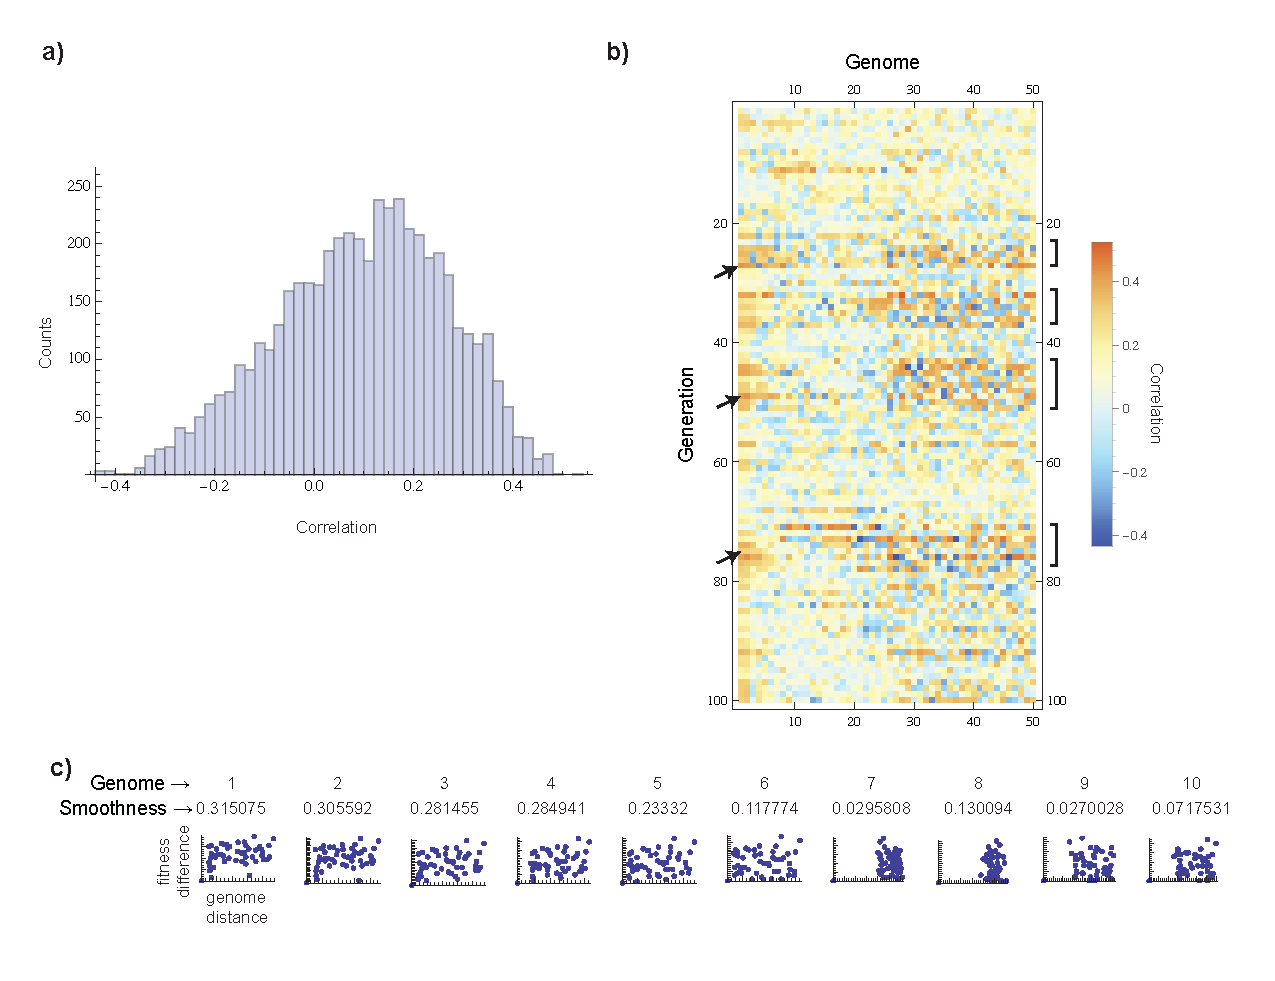
\includegraphics[width=\textwidth]{figures/smoothness/smoothness.pdf}
	\caption{Smoothness of Fitness Landscape. \subfigure{a} Histogram showing the distribution of values for $\rho^f$ over all genomes in all generations of an evolutionary process. \subfigure{b} Plot showing $\rho_i^f$ for each genome in the first 100 generations of an evolutionary process; each row is a different generation, and cells within a row are distinct genomes, ordered left-to-right by decreasing fitness. Colors show the values of $\rho_i^f$ for each cell.  \subfigure{c} Series of plots comparing genome distances $\hat{g}_{i,j}$ to fitness distances $\hat{f}_{i,j}$, for $i = 1, 2, \ldots 10$ (the 10 genomes with the highest fitnesses) in generation \#77.  }
	\label{fig:smoothness}
\end{figure*}

\begin{figure*}
	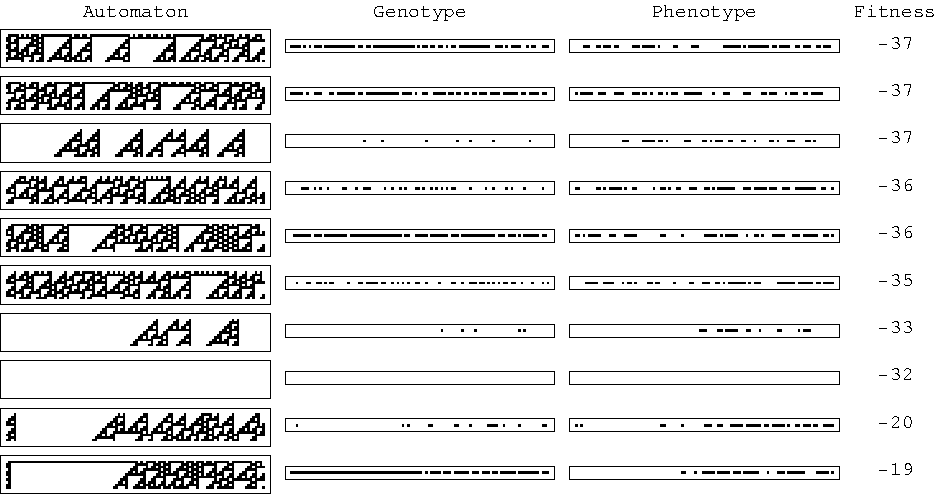
\includegraphics[width=\textwidth]{figures/smoothness/different-genotype-similar-performance.pdf}
	\caption{Different genotypes with similar performances. The 10 fittest genotypes in an evolutionary process whose target structure was half 0's, half 1's. In this process, the genotype-phenotype mapping was achieved by running the automaton for 10 steps. These genotypes are selected from a pool of 100 genotypes, evolved for 1000 selection cycles. }
	\label{fig:similar-performance}
\end{figure*}


% =============================================================================
\section{Discussion}

% TODO: discuss evolutionary pattern formation results

The question of fitness landscape smoothness is central to the question of whether a particular search problem is amenable to solution by an evolutionary algorithm at all. We observe that the fitness landscape defined by our evolutionary processes, while not generally smooth, has regions of local smoothness. On the one hand, this is surprising, given the chaotic nature of Rule 110 and the undecidable mapping between inputs and outputs for generalized 110 processes (e.g. cellular automata running Rule 110, whose stopping conditions are determined by automaton output). On the other hand, biological systems are constantly solving an evolutionary problem with a highly non-smooth fitness landscape---many random mutations are lethal or result in drastic changes in fitness. Epistasis (multiple mutations having non-additive effects) and pleiotropy (individual genes influencing multiple, unrelated phenotypic traits) create the potential for significant jumps in fitness with small mutations to a genome. \cite{Ostman:2012iq} However, certain properties of the genotype-to-phenotype mapping (for instance, degeneracy in the genetic code, allowing for mutations that produce identical or similar peptide sequences) allow for a high degree of local smoothness.  Further, features of the selection process allow populations of various sizes to cross fitness valleys, even in the absence of sexual reproduction. \cite{Weissman:2009dh} Our observation suggests that certain search problems, despite having a complex mapping from genotype-to-phenotype, may have simple formulations that allow for ``smooth enough'' fitness landscapes for evolutionary search. 

% =============================================================================
\section{Conclusion}

There is room for much further work in the exploration of the shape and smoothness of the fitness landscape. A more systematic investigation of the genotypes with locally smooth neighbors could yield interesting insights into the space of possible Rule 110 inputs. We have made qualitative observations about the patterns of smoothness within and across generations (e.g. that high-fitness genomes exist in smoother regions, and that episodic behavior occurs in the smoothness of generations); it would be interesting and fruitful to test these hypotheses by bringing statistical tests to bear on larger experiments than were attempted here.

% =============================================================================
\section{Contributions}

C. G. wrote the code for the evolutionary algorithm, and performed the analysis of the fitness landscape smoothness. A. G. wrote the code for the cellular automaton and performed simulations to test evolutionary pattern formation.  

% =============================================================================

\bibliography{library}
\bibliographystyle{ieeetr}
\end{document}